\documentclass[1pt, a4paper]{article}

%Texte et LuaLaTeX
\usepackage{luatextra}
\usepackage{polyglossia}
\setmainfont{Libertinus Serif}
% \setmainfont{Arial}
\usepackage[locale=FR]{siunitx}
\usepackage{booktabs}
\usepackage{xspace}
\usepackage{pict2e}
\usepackage{fullpage}
\usepackage{eso-pic}

\setlength{\unitlength}{1cm}

%Paramètres de langue
\setdefaultlanguage{english}
\setotherlanguage{french}

% Marges du document
\usepackage[lmargin=3cm, rmargin=2cm, vmargin=2.5cm]{geometry}

% En-tête et pieds de page
\iffalse
\usepackage{fancyhdr}
\pagestyle{fancy}
\fancyhead[R]{\textsc{sous-titre}}
\fancyhead[L]{Paradis Enzo}
\renewcommand{\footrulewidth}{1pt}
\fancyfoot[L]{catégorie}
\fancyfoot[R]{\thepage}
\fancyfoot[C]{}
\setlength{\headheight}{15pt}
\fi

%Packages maths
\usepackage{amsmath,amsfonts,amssymb,amsthm}
\usepackage{unicode-math}
%Autres
\usepackage{graphicx} %Insertion d'images
\usepackage{array}    %mise en forme tableau
\usepackage{hyperref} %liens internes au document
\usepackage{lipsum}   %lipsum
\usepackage{caption}  %caption sans figure
\usepackage{xcolor}
\usepackage{enumitem}
\usepackage{multicol}
\usepackage{subcaption}
\usepackage{tikz}
\usepackage{bbold}
\usepackage{appendix}
\usepackage{booktabs}
%code
\usepackage{minted}

%Optimisation
\renewcommand{\arraystretch}{1.2}
\renewcommand{\thesection}{\Roman{section}}

\numberwithin{equation}{section} 

\newcommand{\HRule}{\rule{\linewidth}{0.5mm}}
\newcommand{\blap}[1]{\vbox to 0pt{#1\vss}}
\newcommand{\tabitem}{~~\llap{\textbullet}~~}

\newcommand\PlaceFigure[3]{%
  \put(\LenToUnit{\dimexpr\paperwidth-#1},\LenToUnit{\dimexpr\paperheight-#2}){\blap{\llap{#3}}}%
}

\newcommand{\maketitlepage}{
\begin{titlepage}

% Add figure to titlepage
%   \AddToShipoutPicture{
%     }
 
    \begin{center}
        \huge\textbf{The Kuramoto Model}\\
        \large\textbf{Technical report for python numerical project}\\
        \vspace*{0.5cm}
        \large{Paradis Enzo}\\
        Student at the university of Bourgogne Franche-Comté\\
        Master CompuPhys - $1^{st}$ year\\
        \vspace*{1cm}
% You can add text here

    \end{center}
  
 
\end{titlepage}
\ClearShipoutPicture
\newpage}

\DeclareMathOperator{\e}{e}
\renewcommand{\exp}[1]{\e^{#1}}
\renewcommand{\vec}[1]{\overrightarrow{#1}}
\newcommand{\deriv}[1]{\mathrm{d}#1\\}
\newcommand{\moy}[1]{\ensuremath{\langle\;#1\;\rangle}\xspace}
\newcommand{\real}{\mathbb{R}}
\newcommand{\intg}{\mathbb{N}}
\newcommand{\oone}{\mathbb{1}}
\newcommand{\Ha}{\mathcal{H}}
\newcommand{\colVec}[4]{
    \begin{pmatrix} 
      #1\\ 
      #2\\
      #3\\
      #4
    \end{pmatrix}}
\newcommand{\rawVec}[4]{
    \begin{pmatrix} 
      #1 & #2 & #3 & #4
    \end{pmatrix}}
\newcommand*{\calVec}[4]{ 
    \left\lvert
      \begin{matrix} 
        #1\\
        #2\\
        #3\\
        #4
      \end{matrix}  
    \right.
  }
\newcommand{\derive}[2]{\dfrac{\deriv{#1}}{\deriv{#2}}}
\newcommand{\partd}[2]{\dfrac{\partial #1}{\partial #2}}
\newcommand{\ket}[1]{\ensuremath{|#1\rangle}\xspace}
\newcommand{\bra}[1]{\ensuremath{\langle #1|}\xspace}
\newcommand{\braket}[2]{\ensuremath{\langle #1 | #2 \rangle}\xspace}
\newcommand{\Braket}[3]{\ensuremath{\bra{#1}#2\ket{#3}}\xspace}
\newcommand{\abs}[1]{\ensuremath{\left|#1\right|}\xspace}
  %
\definecolor{couleur_lien}{RGB}{0, 102, 204}
\definecolor{couleur_lien2}{RGB}{0, 0, 254}
\hypersetup{
	colorlinks=true,
    linkcolor={couleur_lien2},
    citecolor={couleur_lien2},
    urlcolor={couleur_lien2}}

\unimathsetup{math-style=TeX}
\setmathfont{Libertinus Math}




\begin{document}
\maketitlepage
\tableofcontents
\newpage
\noindent
The Kuramoto Model (Yoshki Kuramoto) is a mathematical model that describes the syncronization of coupled oscillators. This program, written by myself, Paradis Enzo, is based on this model to describe a set of 2D-coupled oscillators in various cases. In particular to reproduce data obtain in the case of the coupled arrays of Josephson junctions \cite{josephson}. This program was edited for the last time the 10/23/2020. It was written in the language python 3 under ubuntu, so you just have to use \mintinline{shell}{python3} to execute it. There are 6 files. The first one is the main file, \mintinline{shell}{main.py}, it is the only one you have to execute, you could have to comment or uncomment some lines. Instead of that you just have to edit one file, the settings file, \mintinline{shell}{settings.py} were you can find all the settings. Then you have the kuramoto file, \mintinline{shell}{kuramoto.py}, where you can find the \py{class KuramotoModel} which contains all the functions related with the model or the verifications. The data file, \mintinline{shell}{data.py}, contains the \py{class Data}, which is used to manage data. The graphs file, \mintinline{shell}{graphs.py}, with the \py{class Graphs} manages the displaying of the results. And the integrator file, \mintinline{shell}{integrator.py}, where you can find the \py{class Integration}, which contains the three integrators : Euler, RK2, RK4. There is also the parameters directory which is important to save data.You can find all this files on \href{https://github.com/faucheresse/swimming_pool/tree/main/prog}{github}.
\section{Functional requirement of the program}
\label{sec:1}
\noindent
All the functions which are used for the computing or the displaying of the results are called in the main file. At first there are the functions wich create the initial values in respect of the parameters set in the settings file, then this values are stocked in data (.dat) files in a directory named "parameters". With these data files, we don't have to repeat the calculations every time we want to test something. Then you have the functions that compute the results (the phase of the oscillators, the complex mean average, and the Shannon entropy), wich are stocked in data files in the same directory. And finally there are the functions that display the graphs by using the module \py{matplotlib.pyplot}. In this section we will describe the functions that create data files and their datas. Firstly the initial datas are created throught the \py{class Data} wich is in the data file. Finally the computing of the other values is in the \py{class KuramotoModel} wich is in the kuramoto file.
\subsection{The initialisation of data}
\label{subs:1.1}
The initial datas are created by the function: \py{data.init_data(state)}. You can choose if you want to create new initial datas by changing the boolean value of the \py{newData=False} variable in the settings file.
\begin{table}[htbp]
    \begin{center}
        \begin{tabular}{p{0.3\linewidth} p{0.3\linewidth} p{0.3\linewidth}} \toprule
            \multicolumn{3}{c}{\py{data.init_data(state="random")}}\\
            \midrule
            \hfil Description & \hfil Input & \hfil Output\\
            \cmidrule(r){1-1} \cmidrule{2-2} \cmidrule(l){3-3}
           
            This function is using to create initial values, stocked in data files in the directory parameters, according to the value of the argument \py{state} set by default to \py{state="random"}. You can create data for random, chimera, inverse, or josephson states. &
            The argument \py{state} is a \py{string}. By default it takes the value \py{"random"} but you can give it these values:\begin{itemize}[leftmargin=15pt]
            \setlength{\itemsep}{0pt}
            \item \py{"random"}
            \item \py{"chimera"}
            \item \py{"inverse"}
            \item \py{"josephson"}
            \end{itemize}
            & This function will retrieve six data file in the parameters directory, computing in according to the \py{state} argument.
            The data files are: \begin{itemize}[leftmargin=15pt, itemsep=0pt]
            \item \py{"omega.dat"}
            \item \py{"theta0.dat"}
            \item \py{"K.dat"}
            \item \py{"eta.dat"}
            \item \py{"alpha.dat"}
            \item \py{"tau.dat"}
            \end{itemize}\\
            \bottomrule
        \end{tabular}
    \end{center}
    \caption{function data.init\_data()}
    \label{tab:init_data}
\end{table}\\
Each \py{state} create six variables, wich are defined as follows:
\begin{itemize}
        \item $\omega$ is a list of real of size N. It contains the natural oscillations of each oscillators.
        \item $\theta_0$ is a list of real of size N. It contains the intial phase of each oscillators. So at the $\theta^i(t=t_0)$.
        \item $K$ is a matrix of real of size N$\times$N. It contains the coupling coefficients between each oscillators depending on the nearest neighbour. The nearest neighbour of an oscillator are defined by M in the settings file. It is set as $30\%$ of the totality of the oscillators, you can change it. 
        \item $\alpha$ is a matrix of real of size N$\times$N. It is the dephasing matrix of the coupling.
        \item $\tau$ is a matrix of real of size N$\times$N. It is the delay matrix.
        \item $\eta$ is a matrix of real of size N$\times$T. It is the representations of external noises for each oscillators at each time $t\in ]0, T[$.
\end{itemize}
They are different for each state, you can see their definitions in the tables \ref{tab:states1} and \ref{tab:states2}. The function \py{uniform()} is from the module \py{random}, and provide random real numbers with uniform distribution, in the range given. The function \py{randint()} do the same things but for integers.
\begin{table}[htbp]
    \begin{center}
        \begin{tabular}{p{0.40\linewidth} p{0.40\linewidth}} \toprule
            \hfil \py{"random"} & \hfil \py{"chimera"}\\
            \cmidrule(r){1-1} \cmidrule(l){2-2}
            This \py{state} represent the case with random values defined by:
            \begin{itemize}[leftmargin=15pt, itemsep=0pt]
                \item $\omega^i=uniform(0, 3)$
                \item $\theta_0^i=uniform(0, \dfrac{2}{\pi})$
                \item $K^i_j=uniform(0, 1e10)$
                \item $\eta^i_j=uniform(0, 0.5)$
                \item $\alpha^i_j=uniform(0, \dfrac{2}{\pi})$
                \item $\tau^i_j=randint(0, N//2)$
            \end{itemize}
            &This \py{state} represent the case of a quantum chimera state\cite{chimera} defined by:
            \begin{itemize}[leftmargin=15pt, itemsep=0pt]
               \item $\omega^i=0.2 + i * 0.4 * sin(\dfrac{i^2 * \pi}{(2 * N^2)})$
               \item $\theta_0^i=uniform(0, \dfrac{2}{\pi})$
               \item $K^i_j=uniform(0, 1e10)$
               \item $\eta^i_j=uniform(0, 0.5)$
               \item $\alpha^i_j=1.46$
               \item $\tau^i_j=randint(0, N//2)$
            \end{itemize}\\
            \bottomrule
        \end{tabular}
    \end{center}
    \caption{\py{states}}
    \label{tab:states1}
\end{table}
\begin{table}[htbp]
    \begin{center}
        \begin{tabular}{p{0.40\linewidth} p{0.40\linewidth}} \toprule
            \hfil \py{"inverse"} & \hfil \py{"josephson"}\\
            \cmidrule(r){1-1} \cmidrule(l){2-2}
            This \py{state} represent the case with the coupling matrix defined by the inverse of the distance between two oscillators, and the delay matrix is proportionnal to this distance. 
            \begin{itemize}[leftmargin=15pt, itemsep=0pt]
                \item $\omega^i=uniform(0, 3)$
                \item $\theta_0^i=uniform(0, \dfrac{2}{\pi})$
                \item \begin{equation*}
                K^i_j=\left\{\begin{array}{ll}
                    \dfrac{1}{\abs{i-j}}\;if\;\abs{i-j} \neq 0\\
                    1e20\;otherwise
                \end{array}\right.
            \end{equation*}
                \item $\eta^i_j=uniform(0, 0.5)$
                \item $\alpha^i_j=1.46$
                \item $\tau^i_j=\abs{i-j}$
            \end{itemize}
            &This \py{state} represent the case of the array of Josephson, data were drawn from this article \cite{josephson}. Their datas are defined by:
            \begin{itemize}[leftmargin=15pt, itemsep=0pt]
               \item $\omega^i=0.2 + 0.4i\times sin(\dfrac{i^2\pi}{(2N^2)})$
               \item $\theta_0^i=uniform(0, \dfrac{2}{\pi})$
               \item $K^i_j=\dfrac{Nr\omega^{i^2}2\e/(\hbar rI_b)-\omega^i}{\sqrt{(L\omega^{i^2} - 1/C)^2 + \omega^{i^2}(R+rN)^2 }}$
               \item $\eta^i_j=uniform(0, 0.5)$
               \item $cos(\alpha^i_j)=\dfrac{L\omega^{i^2} - 1/C}{\sqrt{(L\omega^{i^2} - 1/C)^2 + \omega^{i^2}(R+rN)^2 }}$
               \item $\tau^i_j=randint(0, N//2)$
            \end{itemize}\\
            \bottomrule
        \end{tabular}
    \end{center}
    \caption{\py{states}}
    \label{tab:states2}
\end{table}
\newpage
\noindent
For each \py{state} choosen you have to define in the settings file the parameters \py{Nr} and \py{Nc}, to define the geometry of the system. \py{Nr} define the number of rows and \py{Nc} the number of columms, so \py{N=Nr*Nc} is the number of oscillators that you have. For example if you choose \py{N=12} in the geometry \py{Nr=3, Nc=4}, you will have this configuration:\\
\begin{figure}[htbp]
    \centering
    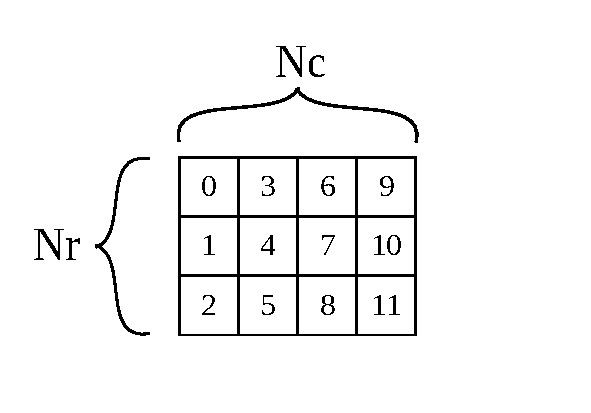
\includegraphics[scale=0.8]{figure/os_table.pdf}
    \caption{Configuration of the oscillators for \py{Nr=3, Nc=4}}
    \label{fig:os_table}
\end{figure}\\
\noindent
The labels in the Figure are the labels of the oscillators. If you put a non-positive number you will have some issues, the program will not work. So be careful to respect the physics of the system.
\subsection{The computing functions}
\label{subs:1.2}
\noindent
There are three computing functions that are imported from the \py{class KuramotoModel}, by the object \py{kuramoto}. You can choose if you want to compute new datas by changing the boolean value of the \py{newComputing=False} variable in the settings file.
\begin{table}[htbp]
    \begin{center}
        \begin{tabular}{p{0.3\linewidth} p{0.3\linewidth} p{0.3\linewidth}} \toprule
            \multicolumn{3}{c}{\py{kuramoto.integrate(f, theta0, tf=100, integrator="RK4")}}\\
            \midrule
            \hfil Description & \hfil Input & \hfil Output\\
            \cmidrule(r){1-1} \cmidrule{2-2} \cmidrule(l){3-3}
           
            This function compute integrates the function \py{f}, with the initial vector \py{theta0} during a time \py{tf}, set by default to \py{tf=100} with 1000 values(T), using the integrator, set by default to \py{integrator="RK4"}&\vspace*{-8pt}
            \begin{itemize}[leftmargin=15pt, itemsep=0pt, topsep=0pt]
            \item \py{f} is the function to be integrated, such that $f:\real^n  \rightarrow  \real^n$
                \item \py{theta0} is the initial vector, such that $\theta_0 \in    \real^n$. So it has to be a list of real of size N
                \item \py{tf} is the duration of the integration. Set to 100 by default. It is an integer
                \item \py{integrator} is the integrator that you want to choose. It can take only this string values: \py{"Euler"}, \py{"RK2"}, \py{"RK4"}. Among the three integrators, RK4 is the one losing the least energy the longer the integration lasts, therefore it is the default value.
            \end{itemize}
            & This function will retrieve two data files in the parameters directory.
            \begin{itemize}[leftmargin=15pt, itemsep=0pt, topsep=0pt]
                \item \py{"theta.dat"} : contains a matrix of real of size N$\times$T. It is used like a list of vectors. Each vector contains the phase of each oscillators at one time, labeled in the same way as the \autoref{fig:os_table}. So the matrix represent the evolution over time of this vector.
                \item \py{"t.dat"} : contains a list of real of size T, defined by \py{linspace(0, tf, T)}. \py{linspace()} is a function added by \py{numpy}.
            \end{itemize}\\
            \bottomrule
        \end{tabular}
    \end{center}
    \caption{function kuramoto.integrate()}
    \label{tab:integrate}
\end{table}
\newpage
\begin{table}[htbp]
    \begin{center}
        \begin{tabular}{p{0.3\linewidth} p{0.3\linewidth} p{0.3\linewidth}} \toprule
            \multicolumn{3}{c}{\py{kuramoto.orders()}}\\
            \midrule
            \hfil Description & \hfil Input & \hfil Output\\
            \cmidrule(r){1-1} \cmidrule{2-2} \cmidrule(l){3-3}
           
            This function computes the orders parameters $R$ and $\Phi$, of the $\theta^i$ over the time, by the relation : $R\e^{\i\Phi} = \frac{1}{N}\sum^N_{i=1}\e^{\i\theta^i}$, for one time.&
            There are no arguments to this function because it takes only data files. It takes the theta file and the t file, see \autoref{tab:integrate}.
            &
            This function will retrieve two data files in the parameters directory.
            \begin{itemize}[leftmargin=15pt, itemsep=0pt, topsep=0pt]
                \item \py{"R.dat"} : It contains a list of real of size T. \py{R} represents the complex mean of magnitudes of the $\theta^i$ over the time.
                \item \py{"phi.dat"} : It contains a list of real of size T. \py{phi} represents the complex mean of angles of the $\theta^i$ over the time.
            \end{itemize}\\
            \bottomrule
        \end{tabular}
    \end{center}
    \caption{function kuramoto.orders()}
    \label{tab:orders}
\end{table}
\begin{table}[htbp]
    \begin{center}
        \begin{tabular}{p{0.3\linewidth} p{0.3\linewidth} p{0.3\linewidth}} \toprule
            \multicolumn{3}{c}{\py{kuramoto.shannon_entropies()}}\\
            \midrule
            \hfil Description & \hfil Input & \hfil Output\\
            \cmidrule(r){1-1} \cmidrule{2-2} \cmidrule(l){3-3}
           
            This function computes the Shannon entropy over the time of $\theta$. So for each vector of the list of vectors \py{theta}&
            There are no arguments to this function because it takes only data files. It takes the theta file and the t file, see \autoref{tab:integrate}.
            &
            This function will retrieve two data files in the parameters directory.
            \begin{itemize}[leftmargin=15pt, itemsep=0pt, topsep=0pt]
                \item \py{"S.dat"} : It contains a list of real of size T. \py{S} represents the Shannon entropy over the time of each vector of \py{theta}
            \end{itemize}\\
            \bottomrule
        \end{tabular}
    \end{center}
    \caption{function kuramoto.shannon\_entropies()}
    \label{tab:shannon}
\end{table}
\noindent
To summarize in the main file there are 4 functions that are called for the computing. The first one is for initializing data according to the state choosed by the user. The following three are here to compute the main datas by using the Kuramoto model. You can choose if you want to initialized new datas (\ref{tab:init_data}) or do a new computing (\ref{tab:integrate}, \ref{tab:orders} \& \ref{tab:shannon}) by modifying the logical variables (\py{newData}, \py{newComputing}) in the settings file. In this file you can modify the \py{state} variable (\ref{tab:states1} \& \ref{tab:states2}). You can also modify the geometry of the system by changing \py{Nr} and \py{Nc}, don't forget to redo the initial datas and the computing after that. Be careful not to set the number of rows or columns to a negative or zero number, it wouldn't make any sense. If you want to save or use other files than the predifined one you can modify it in the dictionnary \py{FILE}. You don't have to modify anything else that is not in the settings file. If you do it be careful, because you can break the program. For the rest of the main file there are 12 functions that are here to display the results. The last three are here to create gifs, they are the begining of the gold version. These displaying functions will be explained later.
\newpage
\noindent
\section{Internal structure of the program}
\label{sec:2}
\subsection{Description of the physical model}
\label{subs:2.1}
In this program we had to describe 2D-coupled oscillators and tried to reproduce the results obtain in the article \textit{Frequency locking in Josephson arrays: Connection with the Kuramoto model} \cite{josephson}. So we will use the Kuramoto Model. Proposed by Yoshiki kuramoto this model is used to describe the syncronization of a large set of coupled oscillators. It is a mathematical model and the form that we have used is : 
\[\dot{\theta}^i(t)=\omega_ i + \dfrac{1}{N}\sum^{N-1}_{j=0}K_{ij}\,sin(\theta^j(t-\tau_{ij})-\theta^i(t)+\alpha_{ij}) + \eta_i(t)\]
where :
\begin{itemize}[itemsep=0pt]
\item $\dot{\theta^i}(t)$ represent the varation of the phase of the i-th oscillator over the time.
\item $\omega_i$ represent the natural frequency of the i-th oscillator.
\item $N$ is the total number of oscillators in the system.
\item $K_{ij}$ is the coupling matrix. It represent the coupling between each oscillators depending on the inverse of the physical distance between them. Sometimes you can consider only the nearest neighbour.
\item $\theta^i$ is the phase of the i-th oscillator.
\item $\tau_{ij}$ is the delay matrix. It is to take into account the phase propagation of the oscillators which have an influence on the i-th oscillator.
\item $\alpha_{ij}$ is the dephasing matrix. It represent the dephasing due of the coupled oscillators.
\item $\eta_i(t)$ represent the influence of the environement, the possible external noises.
\end{itemize}
As you can see this model is pretty complete. The formula is the sum of all the influences due to the environment and the coupled oscillators occuring on each oscillators at a given given time. That why it was chosen to build $\theta$ like a list of vectors.
\subsection{Desciption of the used scientific computation algorithms}
\label{subs:2.2}
During the computation we have used 3 algorithm for the integration of the kuramoto model \ref{subs:2.1}, the Euler, RK2 and RK4 algorithm. But you can choose the one that you want to use. It is recommended to use the RK4 method because it loses less energy over time than the others, so it is more precise but if you want less computing time it is a good thing to try the other. You can see all these integrators in the \py{class Integration} in the integrator file.\\
Let $\theta\in\real^n$ and $f:\real^n  \rightarrow  \real^n$. We wil note $\theta^i$ the i-th component of $\theta$ and $\theta_n$ the vector $\theta$ at the time $t_n$, $\theta_n \equiv \theta(t_n)$. So we have $\theta^i_n$ the i-th component at a time $t_n$ of $\theta$.\\
The Euler and Runge-Kutta methods are integrators of first-order differential equations and are based on the definition of the derivative:
\begin{equation}
\begin{aligned}
    \dot{\theta}(t_n) &= \dfrac{\theta(t_n + h) - \theta(t_n)}{h}\simeq\dfrac{\theta_{n+1} - \theta{n}}{\Delta t}\\
    \iff \theta_{n+1} &= \theta_n + \dot{\theta}(t_n)\Delta t = theta_n + f(\theta_n)\Delta t
\end{aligned}
\end{equation}
with $\Delta t = \dfrac{T}{N_t}$ the step of the simulation ($N_t\in\intg$ the number of steps of the simulation and $T$ the time of the simulation). We need $\Delta t$ sufficiently small so $N_t$ enought large and $T$ sufficiently thin.
\subsubsection{Euler method}


\newpage
\bibliographystyle{plain}
\bibliography{biblio}

\end{document}
